\documentclass[tikz,border=2pt]{standalone}
\usepackage{tikz}
\usepackage{lmodern}
\usetikzlibrary{calc,decorations.pathreplacing}

% Visual conventions follow the existing MRNC TikZ pictures: ordinary
% components use TikZ's normal 0.4pt stroke, with compact TeX labels.
\tikzset{
  nu fibre/.style={
    x=0.78cm,
    y=0.78cm,
    line width=0.4pt,
    line cap=round,
    line join=round
  },
  nu label/.style={
    font=\scriptsize,
    inner sep=1pt
  },
  nu annotation/.style={
    font=\scriptsize,
    inner sep=1pt
  },
  nu dots/.style={
    font=\small,
    inner sep=0pt
  }
}

\begin{document}

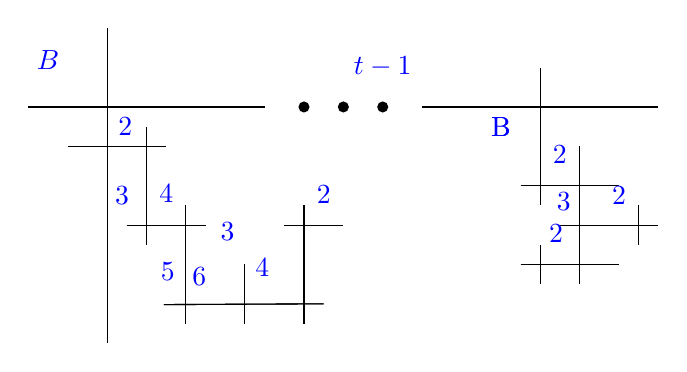
\begin{tikzpicture}
        %chain
  \coordinate (C) at (-2.50, 3.00);
  \coordinate (D) at (-1.50, 3.00);
  \coordinate (A) at (-2.00, 3.00);
  \coordinate (B) at (-1.5, 3.26);
\node[above, text=blue] at (B) {$t-1$};
  \fill[black] (C) circle (2pt);
  \fill[black] (D) circle (2pt);
  \fill[black] (A) circle (2pt);

  %II^*
      \coordinate (1A) at (-5.00, 4.00);
  \coordinate (1B) at (-5.00, 0.00);
  \coordinate (1C) at (-6.00, 3.00);
  \coordinate (1D) at (-3.00, 3.00);
  \coordinate (1E) at (-5.50, 2.50);
  \coordinate (1F) at (-4.25, 2.50);
  \coordinate (1G) at (-4.75, 1.50);
  \coordinate (1H) at (-3.75, 1.50);
  \coordinate (1I) at (-4.28, 0.49);
  \coordinate (1K) at (-2.75, 1.50);
  \coordinate (1L) at (-2.00, 1.50);
  \coordinate (1M) at (-4.50, 2.75);
  \coordinate (1N) at (-4.50, 1.25);
  \coordinate (1O) at (-4.00, 1.75);
  \coordinate (1P) at (-4.00, 0.25);
  \coordinate (1J) at (-2.25, 0.50);
  \coordinate (1S) at (-2.50, 1.75);
  \coordinate (1T) at (-2.50, 0.25);
  \coordinate (1Q) at (-3.25, 1.00);
  \coordinate (1R) at (-3.25, 0.25);
  \coordinate (1U) at (-5.75, 3.35);
  \coordinate (1V) at (-4.77, 2.51);
  \coordinate (1W) at (-4.81, 1.64);
  \coordinate (1X) at (-4.25, 1.66);
  \coordinate (1Y) at (-4.23, 0.67);
  \coordinate (1Z) at (-3.83, 0.61);
  \coordinate (1AA) at (-3.47, 1.18);
  \coordinate (1AB) at (-3.03, 0.72);
  \coordinate (1AC) at (-2.25, 1.65);

 
  \draw (1G) -- (1H);
  \draw (1A) -- (1B);
  \draw (1C) -- (1D);
  \draw (1E) -- (1F);
  \draw (1G) -- (1H);
  \draw (1I) -- (1J);
  \draw (1K) -- (1L);
  \draw (1M) -- (1N);
  \draw (1O) -- (1P);
  \draw (1Q) -- (1R);
  \draw (1I) -- (1J);
  \draw (1S) -- (1T);
  \draw (1Q) -- (1R);
  \node[above, text=blue] at (1U) {$B$};
  \node[above, text=blue] at (1V) {$2$};
  \node[above, text=blue] at (1W) {$3$};
  \node[above, text=blue] at (1X) {$4
$};
  \node[above, text=blue] at (1Y) {$5$};
  \node[above, text=blue] at (1Z) {$6$};
  \node[above, text=blue] at (1AA) {$3$};
  \node[above, text=blue] at (1AB) {$4$};
  \node[above, text=blue] at (1AC) {$2$};

  %IV 
  
  \coordinate (IVSSlA) at (-1.00, 3.00);
  \coordinate (IVSSlB) at (2.00, 3.00);
  \coordinate (IVSSlC) at (0.50, 3.50);
  \coordinate (IVSSlD) at (0.50, 1.75);
  \coordinate (IVSSlE) at (0.25, 2.00);
  \coordinate (IVSSlF) at (1.50, 2.00);
  \coordinate (IVSSlG) at (1.00, 2.50);
  \coordinate (IVSSlH) at (1.00, 0.75);
  \coordinate (IVSSlI) at (0.75, 1.50);
  \coordinate (IVSSlJ) at (2.0, 1.50);
  \coordinate (IVSSlK) at (1.75, 1.75);
  \coordinate (IVSSlL) at (1.75, 1.25);
  \coordinate (IVSSlM) at (0.25, 1.00);
  \coordinate (IVSSlN) at (1.50, 1.00);
  \coordinate (IVSSlO) at (0.50, 1.25);
  \coordinate (IVSSlP) at (0.50, 0.75);
  \coordinate (IVSSlR) at (0.75, 2.16);
  \coordinate (IVSSlQ) at (0, 2.50);
  \coordinate (IVSSlS) at (1.5, 1.64);
  \coordinate (IVSSlU) at (0.8, 1.56);
  \coordinate (IVSSlV) at (0.7, 1.15);


  \draw (IVSSlA) -- (IVSSlB);
  \draw (IVSSlG) -- (IVSSlG);
  \draw (IVSSlG) -- (IVSSlG);
  \draw (IVSSlC) -- (IVSSlD);
  \draw (IVSSlE) -- (IVSSlF);
  \draw (IVSSlG) -- (IVSSlG);
  \draw (IVSSlG) -- (IVSSlH);
  \draw (IVSSlG) -- (IVSSlH);
  \draw (IVSSlI) -- (IVSSlI);
  \draw (IVSSlI) -- (IVSSlJ);
  \draw (IVSSlF) -- (IVSSlF);
  \draw (IVSSlF) -- (IVSSlF);
  \draw (IVSSlK) -- (IVSSlK);
  \draw (IVSSlJ) -- (IVSSlJ);
  \draw (IVSSlJ) -- (IVSSlJ);
  \draw (IVSSlF) -- (IVSSlF);
  \draw (IVSSlK) -- (IVSSlL);
  \draw (IVSSlK) -- (IVSSlL);
  \draw (IVSSlM) -- (IVSSlN);
  \draw (IVSSlI) -- (IVSSlI);
  \draw (IVSSlI) -- (IVSSlI);
  \draw (IVSSlO) -- (IVSSlP);
  \node[above, text=blue] at (IVSSlQ) {B};
  \node[above, text=blue] at (IVSSlR) {$2$};
  \node[above, text=blue] at (IVSSlQ) {B};
  \node[above, text=blue] at (IVSSlS) {$2$};

  \node[above, text=blue] at (IVSSlU) {$3$};
  \node[above, text=blue] at (IVSSlV) {$2$};
\end{tikzpicture}

\end{document}
